 
\section{Implementation}
We use Python for our implementation. So far, our implementation includes several classes
that facilitate the user interface and enables us to play poker with an agent. We describe the
infrastructure here:

\BIT
\item {\tt pokerCards} is a class which consists of cards. Each {\tt pokerCard} has 
two parameters rank and suit.
Rank is a number in $\{2,3,\cdots,14\}$ (where 14 means Ace) and suit is a number in 
$\{1,2,3,4\}$.
\item {\tt deck} is a class which contains a deck of cards. {\tt deck} includes 
{\tt pokerCards} as a subclass and defines methods for shuffle, pop, and peek.
\item {\tt player} consists of player objects. Each object contains information on the player like
the role (small blind or big blind), hole cards, stack (the number of chips), and the set of
possible actions a player can do.
\item {\tt table} is a user interface to show the table, card, players, and status of the game.
\item {\tt handEvaluator} contains functions to evaluate poker hands.
In particular, the method we use is inspired by \ref{ref1}. The idea here is to assign scores to sets of
five, six, or seven cards such that the hand with higher rank has a higher score and equally-ranked
hands have the exact score. Specifically, {\tt hadEvaluator.handEvaluator} function 
receives the hole cards and  
the board (with three to five cards) as its arguments and assigns a real number in $[0,1]$
to the union of hole cards and the board. If {\tt handEvaluator(h1,b) > handEvaluator(h2,b)},
it means that the rank of best five cards in {\tt h1$\cup$b} is higher than the best five cards
in {\tt h2$\cup$b}. Notice that this doesn't mean the {\tt h1} does not have any chance to win.
\EIT
\begin{figure}[h!]
  	\centering
 	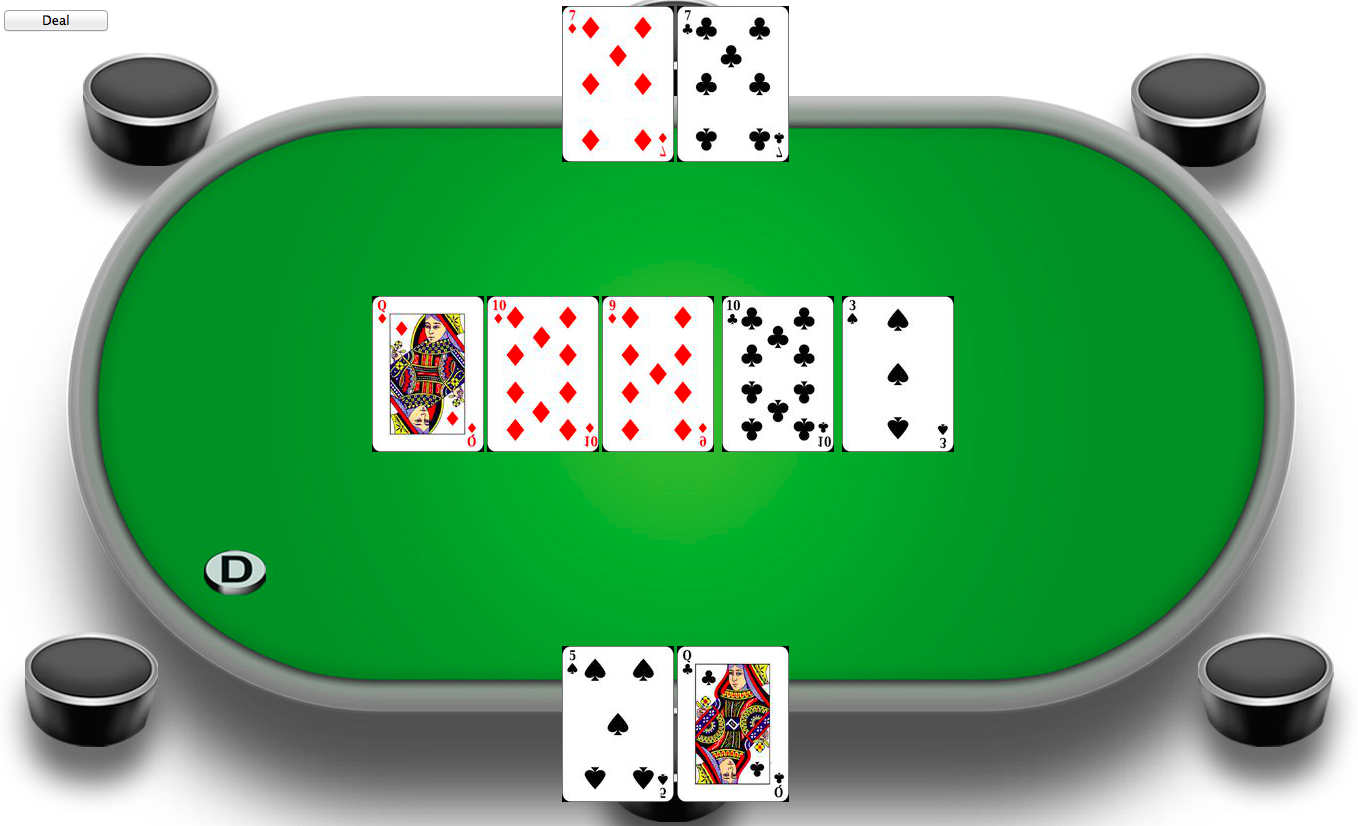
\includegraphics[scale = .3]{table}
	\caption{visual representation of the table}
\end{figure}

In order to decrease the number of states, we are working on {\tt cards abstraction}. The basic
idea is to use abstract class of cards to represent the rank of a hand. For example, if multiple cards
will make a flush, we consider all of them as the same event. We will explain this more in our
final report.

\section{References}
\BIT
\item [1] {S. Ganzfried and T. Sandholm}, {Computing an Approximate Jam/Fold Equilibrium for 3-player No-Limit Texas Holdem Tournaments}
\item [2] {K. B. Korb and A. E. Nicholson and N. Jitnah}, {Bayesian Poker}
\item [3] {The challenge of Poker}
,{D. Billings, A. Davidson, J. Scharffer, D. Szafron}
\item [4] {A heads-up no-limit Texas Hold?em poker player: Discretized betting models and automatically generated equilibrium-finding programs}, {A. Gilpin, T. Sandholm, T. B. Sorensen}
\item [5] http://www.suffecool.net/poker/evaluator.html
\EIT